
\pgfplotsset{compat=1.18}
\usepackage{subcaption}
\usepackage{geometry}
\geometry{a4paper, margin=1in}
\begin{document}

\subsection{Benchmark Railway Network 1}
Figure \ref{fig:network1} presents the results for benchmark network 1
    \centering
    \begin{minipage}[t]{0.3\linewidth}
    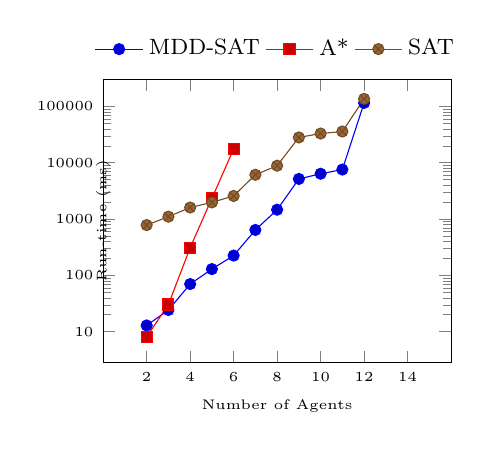
\begin{tikzpicture}
    \pgfplotsset{every axis legend/.append style={
        at={(0.5,1.03)},
        anchor=south
    },
    every axis y label/.append style={
        at={(0.07,0.5)}
    }}
    \begin{axis}[
        xlabel=Number of Agents,
        ylabel=Run-time (ms),
        legend columns=3,
        legend style={draw=none,font=\footnotesize},
        ylabel style={yshift=1mm},
        font=\tiny,
        width=6cm,
        xmin=0, xmax=16,
        ymode=log,
        log ticks with fixed point,
        ymin=0, ymax=300000,
        xtick={2, 4, 6, 8, 10, 12, 14},
        ytick={10, 100, 1000,10000, 100000},
        yticklabels={10, 100, 1000, 10000, 100000},
        minor y tick num=0, % No minor ticks
    ]
     
    \addplot coordinates {
        (2, 12.9)
        (3, 24.3)
        (4, 70.1)
        (5, 129.3)
        (6, 224.8)
        (7, 641.5)
        (8, 1467.0)
        (9, 5160.0) 
        (10, 6383.2)	
        (11, 7581.3)
        (12, 115692.7)
    };
    \addplot coordinates {
        (2, 8.1)
        (3, 30.3) 
        (4, 310.8)
        (5, 2330.6)
        (6, 17561.2)	
    };  
    \addplot coordinates {
        (2, 782.1)
        (3, 1103.5) 
        (4, 1604.9)
        (5, 1977.8)
        (6, 2574.2)	
        (7, 6125.1)
        (8, 8874.9)
        (9, 28192.9) 
        (10, 33074.7)	
        (11, 35925.5)
        (12, 136286.9)
    };  
    \legend{MDD-SAT,A*,SAT,MDD-SAT()}

    
    \end{axis}
\end{tikzpicture}
    \subcaption{\tiny{Run-time for Benchmark Railway Network 1}}
    
    \label{fig:network1_a}
    \end{minipage}
      \hspace{0.6cm} %设置水平间隙
    \begin{minipage}[t]{0.3\linewidth}
    \begin{tikzpicture}
    \pgfplotsset{every axis legend/.append style={
    at={(0.5,1.03)},
    anchor=south},every axis y label/.append style={at={(0.07,0.5)}}}
    \begin{axis}[
  
    legend columns=3,
    legend style={font=\tiny},
    ylabel style={yshift=1mm},
    font=\tiny,
    width=6cm, 
    ymode=log,
    log ticks with fixed point,
    ytick={10000, 100000,1000000},
    yticklabels={10000, 100000,1000000}]
    \addplot coordinates {
    (2, 19168.3)
    (3, 20104.1)
    (4, 21844.4)
    (5, 23592.9)
    (6, 24300.4)
    (7, 27649.1)
    (8, 31539.2)
    (9, 39522.6)
    (10, 43184.5)
    (11, 46512.2)
    (12, 81320.0)
    };
    \addplot coordinates {
    (2, 3980.2)
    (3, 5012.0)
    (4, 15608.5)
    (5, 80836.7)
    (6, 539524.6)
    };  
    \addplot coordinates {
    (2, 52292.8)
    (3, 69268.4)
    (4, 99265.4)
    (5, 124864.9)
    (6, 151392.1)
    (7, 372860.2)
    (8, 516876.8)
    (9, 1544172.2)
    (10, 1726744.1)
    (11, 1882848.5)
    (12, 7141497.7)
    };
    \end{axis}
    \end{tikzpicture}
    \subcaption{\tiny{Memory Consumption for Benchmark Railway Network 1}}
    \label{fig:network1_b}
    \end{minipage}  
    \hspace{0.5cm} %设置水平间隙
    \begin{minipage}[t]{0.3\linewidth}
    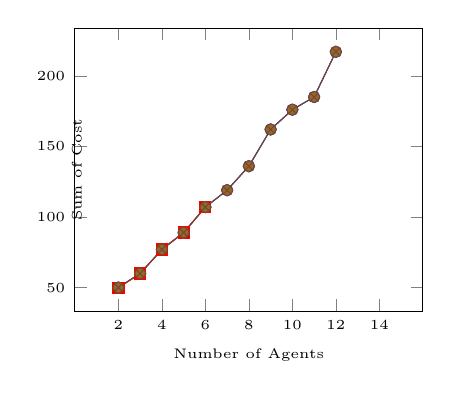
\begin{tikzpicture}
    \pgfplotsset{every axis legend/.append style={
    at={(0.5,1.03)},
    anchor=south},every axis y label/.append style={at={(0.07,0.5)}}}
    \begin{axis}[
        xlabel=Number of Agents,
        ylabel=Sum of Cost,
        legend columns=3,
        xmin=0, xmax=16,
        xtick={2, 4, 6, 8, 10, 12, 14},
        legend style={font=\tiny},
        ylabel style={yshift=1mm},
        font=\tiny,width=6cm]
        
    \addplot coordinates {
        (2, 50)
        (3, 60)
        (4, 77) 
        (5, 89)
        (6, 107)
        (7, 119) 
        (8, 136) 
        (9, 162) 
        (10, 176)
        (11, 185)
        (12, 217)
    };
    \addplot coordinates {
        (2, 50)
        (3, 60)
        (4, 77) 
        (5, 89)
        (6, 107)
    };   
    \addplot coordinates {
        (2, 50)
        (3, 60)
        (4, 77) 
        (5, 89)
        (6, 107)
        (7, 119) 
        (8, 136) 
        (9, 162) 
        (10, 176)
        (11, 185)
        (12, 217)
    };
    \end{axis}
    \end{tikzpicture}
    \subcaption{\tiny{Sum of Cost for Benchmark Railway Network 1}}
    \label{fig:network1_c}
    \end{minipage}
    \caption{Test Results on Benchmark Railway Network 1}
    \label{fig:network1}
\end{figure*}


\subsection{Benchmark Railway Network 2}
For benchmark network 2, the results are illustrated in Figure \ref{fig:network2}. 

\begin{figure*}[ht]
    \centering
    \begin{minipage}[t]{0.3\linewidth}
    \begin{tikzpicture}
    \pgfplotsset{every axis legend/.append style={
        at={(0.5,1.03)},
        anchor=south
    },
    every axis y label/.append style={
        at={(0.07,0.5)}
    }}
    \begin{axis}[
        xlabel=Number of Agents,
        ylabel=Run-time (ms),
        legend columns=3,
        legend style={draw=none,font=\footnotesize},
        ylabel style={yshift=1mm},
        font=\tiny,
        width=6cm,
        xmin=0, xmax=14,
        ymode=log,
        log ticks with fixed point,
        ymin=0, ymax=300000,
        xtick={2, 4, 6, 8, 10, 12, 14},
   
    ]
     
    \addplot coordinates {
        (2, 76.9)
        (3, 174.2)
        (4, 316.1)
        (5, 431.0)
        (6, 3760.8)
        (7, 8508.2)
        (8, 10420.3)
        (9, 15740.7)
        (10, 39737.4)
        (11, 57994.2)
        (12, 117255.3)
    };
    \addplot coordinates {
        (2, 28.0)
        (3, 252.1) 
        (4, 1752.6) 
        (5, 14429.9)
    }; 
    \addplot coordinates {
        (2, 10294.9)
        (3, 11626.2)
        (4, 12031.3)
        (5, 18060.0)
        (6, 62328.1)
        (7, 100998.4)
        (8, 142114.7)
        (9, 235353.3)
    };
    \legend{MDD-SAT,A*,SAT,MDD-SAT)}
    \end{axis}
\end{tikzpicture}
    \subcaption{\tiny{Run-time for Benchmark Railway Network 2}}
    \label{fig:network2_a}
    \end{minipage}
      \hspace{0.6cm} %设置水平间隙
    \begin{minipage}[t]{0.3\linewidth}
    \begin{tikzpicture}
    \pgfplotsset{every axis legend/.append style={
    at={(0.5,1.03)},
    anchor=south}, every axis y label/.append style={at={(0.07,0.5)}}}
    \begin{axis}[
    xlabel=Number of Agents,

    legend style={font=\tiny},
    ylabel style={yshift=1mm},
    font=\tiny,
    width=6cm, 
    ymode=log,
    log ticks with fixed point,
    ytick={10000, 100000,1000000},
    yticklabels={10000, 100000,1000000}]
    \addplot coordinates {
    (2, 23144.5)
    (3, 24524.6)
    (4, 26984.6)
    (5, 28392.7)
    (6, 38724.9)
    (7, 44840.9)
    (8, 51272.0)
    (9, 59744.8)
    (10, 74816.9)
    (11, 87116.7)
    (12, 88048.4)
    };
    \addplot coordinates {
    (2, 4680.7)
    (3, 13512.8)
    (4, 63576.9)
    (5, 468084.4)
    };
    \addplot coordinates {
    (2, 287916.3)
    (3, 345520.4)
    (4, 386996.6)
    (5, 578876.1)
    (6, 1745916.6)
    (7, 2832264.1)
    (8, 3709508.4)
    (9, 6561636.4)
    };   
    \end{axis}
    \end{tikzpicture}
    \subcaption{\tiny{Memory Consumption for Benchmark Railway Network 2}}
    \label{fig:network2_b}
    \end{minipage}  
    \hspace{0.5cm} %设置水平间隙
    \begin{minipage}[t]{0.3\linewidth}
    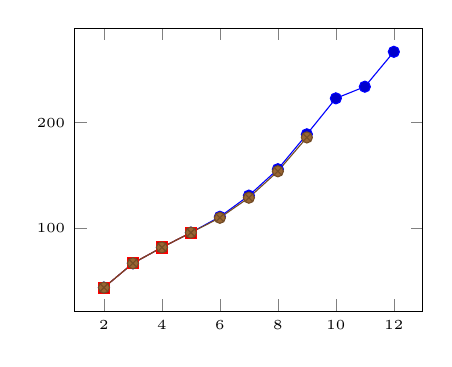
\begin{tikzpicture}
    \pgfplotsset{every axis legend/.append style={
    at={(0.5,1.03)},
    anchor=south},every axis y label/.append style={at={(0.07,0.5)}}}
    \begin{axis}[ xtick={2, 4, 6, 8, 10, 12, 14, 16},
        legend style={font=\tiny},
        ylabel style={yshift=1mm},
        font=\tiny,width=6cm]
        
    \addplot coordinates {
      (2, 44)
        (3, 67)
        (4, 82)
        (5, 96)
        (6, 111)
        (7, 131)
        (8, 156)
        (9, 189)
        (10, 223)
        (11, 234)
        (12, 267)
    };
    \addplot coordinates {
         (2, 44) (3, 67) (4, 82) (5, 96)

    };   
    \addplot coordinates {
        (2, 44)
        (3, 67)
        (4, 82)
        (5, 96)
        (6, 110)
        (7, 129)
        (8, 154)
        (9, 186)
    };
    \end{axis}
    \end{tikzpicture}
    \subcaption{\tiny{Sum of Cost for Benchmark Railway Network 2}}
    \label{fig:network2_c}
    \end{minipage}
    \caption{Test Results on Benchmark Railway Network 2}
    \label{fig:network2}
\end{figure*}

\subsection{Benchmark Railway Network 3}
The results for benchmark network 3, presented in Figure \ref{fig:network3}, follow a similar trend to the previous benchmarks. 
\begin{figure*}[ht]
    \centering
    \begin{minipage}[t]{0.3\linewidth}
    \begin{tikzpicture}
    \pgfplotsset{every axis legend/.append style={
        at={(0.5,1.03)},
        anchor=south
    },
    every axis y label/.append style={
        at={(0.07,0.5)}
    }}
    \begin{axis}[
        xlabel=Number of Agents,
        ylabel=Run-time (ms),cm,
        xmin=0, xmax=14,
        ymode=log,
        log ticks with fixed point,
        ymin=0, ymax=300000,
        xtick={2, 4, 6, 8, 10, 12, 14, 16, 18, 20},
        ytick={10, 100, 1000, 10000, 100000},
        yticklabels={10, 100, 1000, 10000, 100000},
        minor y tick num=0, % No minor ticks
    ]
     
    \addplot coordinates {
        (2, 19.0)
        (3, 110.3) 
        (4, 1701.3) 
        (5, 2404.0) 
        (6, 3448.5) 
        (7, 6356.3) 
        (8, 8558.4)
        (9, 25150.4)
        (10, 33144.1)
        (11, 36726.9)
        (12, 47724.1)
    };
    \addplot coordinates {
        (2, 17.2)
        (3, 143.3) 
        (4, 8571.6) 
    }; 
    \addplot coordinates {
        (2, 652.7)
        (3, 4313.0) 
        (4, 34650.0) 
        (5, 65575.5) 
        (6, 74335.4) 
        (7, 101522.4) 
        (8, 114021.5)
        (9, 174209.2)
        (10, 210077.3)
        (11, 213621.8)
        (12, 228831.9)
    };
    \legend{MDD-SAT,A*,SAT,MDD-SAT)}
    \end{axis}
\end{tikzpicture}
    \subcaption{\tiny{Run-time for Benchmark Railway Network 3}}
    \label{fig:network3_a}
    \end{minipage}
      \hspace{0.6cm} %设置水平间隙
    \begin{minipage}[t]{0.3\linewidth}
    \begin{tikzpicture}
    \pgfplotsset{every axis legend/.append style={
    at={(0.5,1.03)},
    anchor=south}, every axis y label/.append style={at={(0.07,0.5)}}}
    \begin{axis}[
    xlabel=Number of Agents,
    ylabel=Memory Consumption (KB),
 
    log ticks with fixed point,
    ytick={10000, 100000,1000000},
    yticklabels={10000, 100000,1000000}]
    \addplot coordinates {
    (2, 18432.4)
    (3, 20720.7)
    (4, 29064.2)
    (5, 31844.8)
    (6, 35536.8) 
    (7, 39600.6) 
    (8, 43388.8) 
    (9, 59048.8) 
    (10, 62444.5)
    (11, 65536.7)
    (12, 75336.3)
    };
    \addplot coordinates {
    (2,3940.0)
    (3,9208.4)
    (4,324036.9)
    }; 
    \addplot coordinates {
    (2, 71612.3)
    (3, 298824.7)
    (4, 991622.8)
    (5, 1889116.4)
    (6, 2229600.2) 
    (7, 3250968.2) 
    (8, 3738528.8) 
    (9, 5591032.9) 
    (10, 6751596.5)
    (11, 7166500.4)
    (12, 9639560.3)
    };
    \end{axis}
    \end{tikzpicture}
    \subcaption{\tiny{Memory Consumption for Benchmark Railway Network 3}}
    \label{fig:network3_b}
    \end{minipage}  
    \hspace{0.5cm} %设置水平间隙
    \begin{minipage}[t]{0.3\linewidth}
    \begin{tikzpicture}
    \pgfplotsset{every axis legend/.append style={
    at={(0.5,1.03)},
    anchor=south}, every axis y label/.append style={at={(0.07,0.5)}}}
    \begin{axis}[
        xlabel=Number of Agents,
        ylabel=Sum of Cost,
        legend columns=3,
 
        ylabel style={yshift=1mm},
        font=\tiny,width=6cm]
        
    \addplot coordinates {
        (2, 33) 
        (3, 53) 
        (4, 80)
        (5, 107) 
        (6, 131) 
        (7, 156) 
        (8, 177) 
        (9, 200) 
        (10, 221)
        (11, 230)
        (12, 245)
    }; 
    \addplot coordinates {
        (2, 33)
        (3, 51)
        (4, 78)
    };  
    \addplot coordinates {
        (2, 33) 
        (3, 53) 
        (4, 80)
        (5, 107) 
        (6, 131) 
        (7, 156) 
        (8, 177) 
        (9, 200) 
        (10, 221)
        (11, 230)
        (12, 245)
    };  
    \end{axis}
    \end{tikzpicture}
    \subcaption{\tiny{Sum of Cost for Benchmark Railway Network 3}}

    \label{fig:network3}
\end{figure*}

\subsection{Benchmark Railway Network 4}
Figure \ref{fig:network4} presents the results for benchmark network 4. 


\begin{figure*}[ht]
    \centering
    \begin{minipage}[t]{0.3\linewidth}
    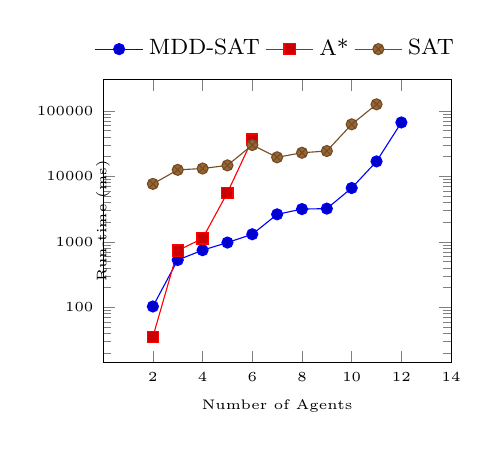
\begin{tikzpicture}
    \pgfplotsset{every axis legend/.append style={
        at={(0.5,1.03)},
        anchor=south
    },
    every axis y label/.append style={
        at={(0.07,0.5)}
    }}
    \begin{axis}[
        xlabel=Number of Agents,
        ylabel=Run-time (ms),
        legend columns=3,
        legend style={draw=none,font=\footnotesize},
        ylabel style={yshift=1mm},
        font=\tiny,
        width=6cm,
        xmin=0, xmax=14,
        ymode=log,
        log ticks with fixed point,
        ymin=0, ymax=300000,
        xtick={2, 4, 6, 8, 10, 12, 14, 16, 18},
        ytick={10, 100, 1000, 10000, 100000},
        yticklabels={10, 100, 1000, 10000, 100000},
        minor y tick num=0, % No minor ticks
    ]
     
    \addplot coordinates {
        (2, 103.2)
        (3, 529.0)
        (4, 746.8)
        (5, 975.6)
        (6, 1307.3)
        (7, 2632.3)
        (8, 3165.9)
        (9, 3218.7)
        (10, 6640.2)
        (11, 16931.3)
        (12, 66582.7)
    };
    \addplot coordinates {
        (2, 35.5) (3, 737.5) (4, 1126.9) (5, 5645.2) (6, 36552.0)	 	

    }; 
    \addplot coordinates {
        (2, 7673.3)
        (3, 12572.2)
        (4, 13173.7)
        (5, 14713.9)
        (6, 30097.3)
        (7, 19540.6)
        (8, 22938.0)
        (9, 24369.1)
        (10, 62290.6)
        (11, 125880.6)
    };
    \legend{MDD-SAT,A*,SAT,MDD-SAT)}
    \end{axis}
\end{tikzpicture}
    \subcaption{\tiny{Run-time for Benchmark Railway Network 4}}
    \label{fig:network4_a}
    \end{minipage}
      \hspace{0.6cm} %设置水平间隙
    \begin{minipage}[t]{0.3\linewidth}
    \begin{tikzpicture}
    \pgfplotsset{every axis legend/.append style={
    at={(0.5,1.03)},
    anchor=south}, every axis y label/.append style={at={(0.07,0.5)}}}
    \begin{axis}[
    xlabel=Number of Agents,
    ylabel=Memory Consumption (KB),
    xmin=0, xmax=14,

    font=\tiny,
    width=6cm, 
    ymode=log,
    log ticks with fixed point,
    ytick={10000, 100000,1000000},
    yticklabels={10000, 100000,1000000}]
    \addplot coordinates {
        (2, 23828.2)
        (3, 28300.0)
        (4, 32180.4)
        (5, 34876.6)
        (6, 40520.0)
        (7, 48428.6)
        (8, 50360.8)
        (9, 54604.4)
        (10, 61980.2)
        (11, 71080.3)
        (12, 95080.7)
    };
    \addplot coordinates {
    (2, 4968.2) (3, 28856.9) (4, 35860.2) (5, 157740.4)	(6, 1134228.4)		

    }; 
    \addplot coordinates {
        (2, 315556.3)
        (3, 529576.7)
        (4, 592784.6)
        (5, 672356.4)
        (6, 767376.3)
        (7, 811268.6)
        (8, 937508.4)
        (9, 1048752.3)
        (10, 2770956.2)
        (11, 8638040.0)
    };
    \end{axis}
    \end{tikzpicture}
    \subcaption{\tiny{Memory Consumption for Benchmark Railway Network 4}}
    \label{fig:network4_b}
    \end{minipage}  
    \hspace{0.5cm} %设置水平间隙
    \begin{minipage}[t]{0.3\linewidth}
    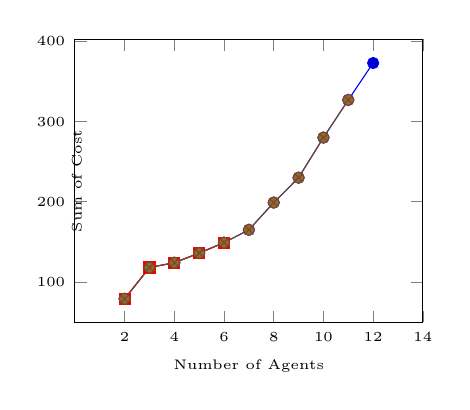
\begin{tikzpicture}
    \pgfplotsset{every axis legend/.append style={
    at={(0.5,1.03)},
    anchor=south}, every axis y label/.append style={at={(0.07,0.5)}}}
    \begin{axis}[
        xlabel=Number of Agents,
        ylabel=Sum of Cost,
        legend columns=3,
        xmin=0, xmax=14,
        xtick={2, 4, 6, 8, 10, 12, 14, 16, 18},
        legend style={font=\tiny},
        ylabel style={yshift=1mm},
        font=\tiny,width=6cm]
        
    \addplot coordinates {
        (2, 79)
        (3, 118)
        (4, 124)
        (5, 136)
        (6, 149)
        (7, 165)
        (8, 199)
        (9, 230)
        (10, 280)
        (11, 327)
        (12, 373)
    };
    \addplot coordinates {
        (2, 79) (3, 118) (4, 124) (5, 136) (6, 149)
    }; 
    \addplot coordinates {
        (2, 79)
        (3, 118)
        (4, 124)
        (5, 136)
        (6, 149)
        (7, 165)
        (8, 199)
        (9, 230)
        (10, 280)
        (11, 327)
    };

    \end{axis}
    \end{tikzpicture}
    \subcaption{\tiny{Sum of Cost for Benchmark Railway Network 4}}
    \label{fig:network4_c}
    \end{minipage}
    \caption{Test Results on Benchmark Railway Network 4}
    \label{fig:network4}
\end{figure*}



\end{document}
